%============================================================
% MTH 112 Project - Polar Coordinates
% Updated 202504
%============================================================

\section{Polar Coordinates} \label{section-polar-coordinates}
In this section, we will learn a completely different way of organizing the coordinate plane: polar coordinates, where a polar point, $(r,\theta)$, has a radius $r$ from the origin and the angle from standard position, $\theta$. We will practice plotting points using polar coordinates, converting between polar coordinates and rectangular coordinates, transforming equations between polar and rectangular forms, and graphing polar equations.

\textbooks{\href{https://openstax.org/books/algebra-and-trigonometry-2e/pages/10-3-polar-coordinates}{10.3}}{\href{https://openstax.org/books/algebra-and-trigonometry-2e/pages/10-4-polar-coordinates-graphs}{10.4}}

\subsection*{Preparation Exercises} \label{preparation-exercises-section-polar-coordinates}

\begin{myPrep}
Answer the following without using a calculator. These questions are intended to check the prerequisite skills needed to complete the rest of the lab.
	\begin{multicols}{2}
		Thinking back to SOHCAHTOA, recall that for a triangle with legs $x$ and $y$ and hypotenuse $r$, as shown in Figure \ref{section-polar-coordinates-prep-triangle}, you know that $\cos(\theta)=\frac{x}{r}$, $\sin(\theta)=\frac{y}{r}$, and $\tan(\theta)=\frac{y}{x}$.
			\begin{center}\captionsetup{type=figure} \captionof{figure}{A right triangle}
				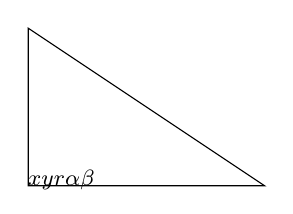
\begin{tikzpicture}[thin] \label{section-polar-coordinates-prep-triangle}
					\coordinate (O) at (0,0);
					\coordinate (A) at (3,0);
					\coordinate (B) at (0,2);
					\draw (O)--(A)--(B)--cycle;
					\footnotesize
					\tkzLabelSegment[below=2pt](O,A){$x$}
					\tkzLabelSegment[left=2pt](O,B){$y$}
					\tkzLabelSegment[above=2pt](A,B){$r$}
					\tkzMarkRightAngle[size=0.5](A,O,B)
					\tkzMarkAngle[size=0.8cm](B,A,O)
					\tkzLabelAngle[pos = 0.6](B,A,O){$\alpha$}
					\tkzMarkAngle[size=0.7cm](O,B,A)
					\tkzLabelAngle[pos = 0.5](O,B,A){$\beta$}
				\end{tikzpicture}
			\end{center}
		\columnbreak
			\begin{enumerate}[itemsep=1.5cm]
				\item Solve $\sin(\theta)=\frac{y}{r}$ for $y$.
				\item Solve $\cos(\theta)=\frac{x}{r}$ for $x$.
				\item What would the Pythagorean Theorem say about the triangle in Figure \ref{section-polar-coordinates-prep-triangle}?
			\end{enumerate}
	\end{multicols}
		% \begin{enumerate}\setcounter{enumi}{2}
		% \end{enumerate}
\end{myPrep}
\vfill

\begin{myPrep}
	What conditions would you need to put on $\theta$, $x$, and $y$ to make the solution to the equation $\tan(\theta)=\frac{y}{x}$ be $\theta=\tan^{-1}\left(\frac{y}{x}\right)$?
\end{myPrep}
\vfill
\vfill

\begin{myPrep}
	Which quadrant are the following angles in, when measured from the standard position.
		\begin{enumerate}
			\begin{multicols}{4}
				\item $\ang{400}$
				\item $\ang{-200}$
				\item $-\frac{7\pi}{6}$
				\item $\frac{17\pi}{3}$
			\end{multicols}
		\end{enumerate}
\end{myPrep}
\vfill

\begin{myPrep}
	Evaluate the expressions using your memorized values on the unit circle.
		\begin{enumerate}
			\begin{multicols}{4}
				\item $\sin(\ang{420})$
				\item $\cos(-\ang{210})$
				\item $\sin\left(-\frac{7\pi}{6}\right)$
				\item $\cos\left(\frac{17\pi}{3}\right)$
			\end{multicols}
		\end{enumerate}
\end{myPrep}
\vfill


%======================================================
\newpage
%======================================================

\subsection*{Practice Exercises} \label{practice-exercises-section-polar-coordinates}


\begin{myPractice}
	Practice plotting points written in polar form. For clarity, a small $_p$ will be written next to polar points to distinguish them from rectangular points, which will be written with a small $_r$ next to them. Label each point.
	\begin{multicols}{2}
		\begin{center}
			\captionsetup{type=figure} \captionof{figure}{A Polar Grid, with Standard Angles and Radii Shown}
			\begin{tikzpicture}
				\begin{axis}[
					xmin=-5,xmax=5,
					ymin=-5,ymax=5,
			       	xtick={1,2,3,4},
			       	ytick={1,2,3,4},
			       	clip=false,
					]
					\addplot[first,line width=1pt,opacity=0.2,samples=2] expression[domain=-5/sqrt(2):5/sqrt(2)]{x};
					\addplot[second,line width=1pt,opacity=0.2,samples=2] expression[domain=-2.5*sqrt(3):2.5*sqrt(3)]{1/sqrt(3)*x};
					\addplot[third,line width=1pt,opacity=0.2,samples=2] expression[domain=-2.5:2.5]{sqrt(3)*x};
					\addplot[first,line width=1pt,opacity=0.2,samples=2] expression[domain=-5/sqrt(2):5/sqrt(2)]{-x};
					\addplot[second,line width=1pt,opacity=0.2,samples=2] expression[domain=-2.5*sqrt(3):2.5*sqrt(3)]{-1/sqrt(3)*x};
					\addplot[third,line width=1pt,opacity=0.2,samples=2] expression[domain=-2.5:2.5]{-sqrt(3)*x};
					\draw[thin,opacity=0.2] (axis cs:0,0) circle [radius=1];
					\draw[thin,opacity=0.2] (axis cs:0,0) circle [radius=2];
					\draw[thin,opacity=0.2] (axis cs:0,0) circle [radius=3];
					\draw[thin,opacity=0.2] (axis cs:0,0) circle [radius=4];
					\draw[thin,opacity=0.2] (axis cs:0,0) circle [radius=5];
				\end{axis}
			\end{tikzpicture}
			\label{fig:section-polar-graph}
		\end{center}
			\columnbreak
			\begin{enumerate}[itemsep=0.3cm]
				\item $\left(4,\frac{\pi}{2}\right)_p$
				% \item $\left(2,\frac{4\pi}{3}\right)_p$
				\item $\left(3,-\frac{\pi}{4}\right)_p$
				\item $\left(-2,\frac{5\pi}{6}\right)_p$
				% \item $(1,\ang{120})_p$
				\item $(2.5,\ang{225})_p$
				\item $(3.5,-\ang{120})_p$
				\item $(-1.5,\ang{270})_p$
			\end{enumerate}
	\end{multicols}
\end{myPractice}

\begin{myPractice}
	Convert the polar points to rectangular form and the rectangular points to polar form. For clarity, a small $_p$ will be written next to polar points to distinguish them from rectangular points, which will be written with a small $_r$ next to them.
		\begin{enumerate}
			\item Find the rectangular coordinates of the polar points. Leave your answers in exact form rather than using your calculator to get a decimal value for the coordinates.
				\begin{enumerate}
					\begin{multicols}{2}
					\item $\left(4,\frac{\pi}{2}\right)_p$
					\vfill
					\item $\left(2,-\frac{4\pi}{3}\right)_p$
					\vfill
					% \item $(-1.5,\ang{270})_p$
					% \vfill
					\end{multicols}
				\end{enumerate}

	%======================================================
	\newpage
	%======================================================

		\item Find the polar coordinates of the rectangular points. 
			\begin{enumerate}
				\begin{multicols}{3}
				\item $(1,1)_r$. Leave your answers in exact form for both the radius and angle.
				\columnbreak
				% \item $\left(-3,\sqrt3\right)_r$. Leave your answers in exact form for both the radius and angle.
				\item $(2,3)_r$. Leave your radius in exact form, but use a calculator to find an approximation of the angle, accurate to three digits behind the decimal place.
				\columnbreak
				\item $(-2,-3)_r$. Leave your radius in exact form, but use a calculator to find an approximation of the angle, accurate to three digits behind the decimal place.
				\columnbreak
				\end{multicols}
			\end{enumerate}
		\end{enumerate}
\end{myPractice}
\vfill

\begin{myPractice}
	Convert equations between polar form and rectangular form. You can graph both the original equation and the polar form equation in Desmos to verify that you have converted correctly.
	\begin{enumerate}
		\item Convert the polar equations to rectangular form. You don't need to solve for a variable, necessarily. %https://www.desmos.com/calculator/abqlib6drm
			\begin{enumerate}
				\begin{multicols}{3}
					\item $r\cos(\theta)=5$ %solution $x=5$
					\item $r=3\sin(\theta)$ %solution $x^2+y^2=3y$
					\item $r=5$ %solution $x^2+y^2=25$
					% \item $r=\frac{3}{\cos(\theta)+2\sin(\theta)}$ %solution $x+2y=3$
				\end{multicols}
			\end{enumerate}
	\vfill
		\item Convert the rectangular equations to polar form. You don't need to solve for a variable, necessarily.
			\begin{enumerate}
				\begin{multicols}{3}
					\item $y=3$ %solution $r=\frac{3}{\sin(\theta)}$
					% \item $y=\frac{2}{x}$ %solution $r=\sqrt{\frac{2}{\sin(\theta)\cos(\theta)}}$
					\item $y=2x+1$ %solution $r=\frac{1}{\sin(\theta)-2\cos(\theta)}$
					\item $x^2+y^2=2x$ %solution $r=2\cos(\theta)$ or $r=0$
				\end{multicols}
			\end{enumerate}
	\vfill
	\end{enumerate}
\end{myPractice}

	%======================================================
	\newpage
	%======================================================

\begin{myPractice}
	Create a graph of the polar functions by filling in the tables and plotting points. Round the values of $r$ to the nearest tenth. Note that Desmos does have polar grid in the settings, and you can graph functions of the form $r=f(\theta)$, where the $\theta$ can be found in the \say{A B C} keyboard. A standardized Desmos template to create this table can be found in the link. \qrcode[height=1cm]{http://tiny.cc/PolarGraphTable}
	\begin{enumerate}
		\item
		\begin{multicols}{2}
			\begin{center}
				\renewcommand{\arraystretch}{1.5} 
				\begin{tabular}{|| c | P{3cm} ||}
					\hline
					$\theta$ & $r=2\sin(\theta)$ \\
					\hline
					$\ang{0}$ & \\ 
					\hline
					$\ang{30}$ & \\ 
					\hline
					$\ang{45}$ & \\ 
					\hline
					$\ang{60}$ & \\ 
					\hline
					$\ang{90}$ & \\ 
					\hline
					$\ang{120}$ & \\ 
					\hline
					$\ang{135}$ & \\ 
					\hline
					$\ang{150}$ & \\ 
					\hline
					$\ang{180}$ & \\
					\hline
				\end{tabular}
			\end{center}
		\columnbreak
			\begin{center}\captionsetup{type=figure} \captionof{figure}{A Polar Grid for the Graph of $r=2\sin(\theta)$}
				\begin{tikzpicture}
					\begin{axis}[
						height=8cm,
						width=8cm,
						xmin=-2.5,xmax=2.5,
						ymin=-2.5,ymax=2.5,
				       	xtick={1,1.5},
				       	ytick={1,1.5},
				       	clip=false,
						]
						\addplot[first,line width=1pt,opacity=0.2,samples=2] expression[domain=-2/sqrt(2):2/sqrt(2)]{x};
						\addplot[second,line width=1pt,opacity=0.2,samples=2] expression[domain=-sqrt(3):1*sqrt(3)]{1/sqrt(3)*x};
						\addplot[third,line width=1pt,opacity=0.2,samples=2] expression[domain=-1:1]{sqrt(3)*x};
						\addplot[first,line width=1pt,opacity=0.2,samples=2] expression[domain=-2/sqrt(2):2/sqrt(2)]{-x};
						\addplot[second,line width=1pt,opacity=0.2,samples=2] expression[domain=-sqrt(3):sqrt(3)]{-1/sqrt(3)*x};
						\addplot[third,line width=1pt,opacity=0.2,samples=2] expression[domain=-1:1]{-sqrt(3)*x};
						\draw[thin,opacity=0.2,dashed] (axis cs:0,0) circle [radius=0.5];
						\draw[thin,opacity=0.2] (axis cs:0,0) circle [radius=1];
						\draw[thin,opacity=0.2,dashed] (axis cs:0,0) circle [radius=1.5];
						\draw[thin,opacity=0.2] (axis cs:0,0) circle [radius=2];
						% \addplot[domain= 0:360] ({cos(x)},{sin(x)+1});
					\end{axis}
				\end{tikzpicture}\label{fig:section-polar-graph-of-2sin}
			\end{center}
		\end{multicols}
		\vfill

		\begin{multicols}{2}
			\item %Issue, fix this item numbering at top.
			\begin{center}
				\renewcommand{\arraystretch}{1.5} 
				\begin{tabular}{|| c | P{3cm} ||}
					\hline
					$\theta$ & $r=2\sin(3\theta)$ \\
					\hline
					$\ang{0}$ & \\ 
					\hline
					$\ang{30}$ & \\ 
					\hline
					$\ang{45}$ & \\ 
					\hline
					$\ang{60}$ & \\ 
					\hline
					$\ang{90}$ & \\ 
					\hline
					$\ang{120}$ & \\ 
					\hline
					$\ang{135}$ & \\ 
					\hline
					$\ang{150}$ & \\ 
					\hline
					$\ang{180}$ & \\
					\hline
				\end{tabular}
			\end{center}
		\columnbreak
			\begin{center}\captionsetup{type=figure} \captionof{figure}{A Polar Grid for a Graph of $r=2\sin(3\theta)$}
				\begin{tikzpicture}
					\begin{axis}[
						height=8cm,
						width=8cm,
						xmin=-2.5,xmax=2.5,
						ymin=-2.5,ymax=2.5,
				       	xtick={1,1.5},
				       	ytick={1,1.5},
				       	clip=false,
						]
						\addplot[first,line width=1pt,opacity=0.2,samples=2] expression[domain=-2/sqrt(2):2/sqrt(2)]{x};
						\addplot[second,line width=1pt,opacity=0.2,samples=2] expression[domain=-sqrt(3):1*sqrt(3)]{1/sqrt(3)*x};
						\addplot[third,line width=1pt,opacity=0.2,samples=2] expression[domain=-1:1]{sqrt(3)*x};
						\addplot[first,line width=1pt,opacity=0.2,samples=2] expression[domain=-2/sqrt(2):2/sqrt(2)]{-x};
						\addplot[second,line width=1pt,opacity=0.2,samples=2] expression[domain=-sqrt(3):sqrt(3)]{-1/sqrt(3)*x};
						\addplot[third,line width=1pt,opacity=0.2,samples=2] expression[domain=-1:1]{-sqrt(3)*x};
						\draw[thin,opacity=0.2,dashed] (axis cs:0,0) circle [radius=0.5];
						\draw[thin,opacity=0.2] (axis cs:0,0) circle [radius=1];
						\draw[thin,opacity=0.2,dashed] (axis cs:0,0) circle [radius=1.5];
						\draw[thin,opacity=0.2] (axis cs:0,0) circle [radius=2];
					\end{axis}
				\end{tikzpicture}\label{fig:section-polar-graph-of-2sin3}
			\end{center}
		\end{multicols}
		\vfill
		\item Visit \href{http://tiny.cc/polar-graphs}{this interactive Desmos graph} and change the values of $a$ and $b$. Find a particular graph that you like, write down it's equation, and discuss what you like about it with your neighbor. \qrcode[height=1cm]{http://tiny.cc/polar-graphs}
		\vfill
	\end{enumerate}
\end{myPractice}

%======================================================
\newpage
%======================================================

\subsection*{Definitions} \label{definitions-section-polar-coordinates}

\begin{myDefinition}[{Polar Functions}]~\\[0.5mm]
	A \textbf{polar function} is usually given in the form $r=f(\theta)$, where $\theta$ is the angle measured from the standard position along the positive $x$-axis, and $r$ is the radius measured from the origin.
\end{myDefinition}

\begin{myDefinition}[{Conversion formulas}]~\\[-0.5mm]
	\begin{itemize}
		\item To convert from rectangular form to polar form, use these two identities.
			\begin{enumerate}[itemsep=0.5cm]
				\item $r=\sqrt{x^2+y^2}$ or $r^2=x^2+y^2$
				\item $\tan(\theta)=\frac{y}{x}$
			\end{enumerate}
		\item To convert from polar form to rectangular form, use these two identities.
			\begin{enumerate}[itemsep=0.5cm]
				\item $x=r\cos(\theta)$
				\item $y=r\sin(\theta)$
			\end{enumerate}
	\end{itemize}
\end{myDefinition}

%======================================================
\newpage
%======================================================

\subsection*{Exit Exercises} \label{exit-exercises-section-polar-coordinates}

\begin{myExit}
	Which quadrant will the polar point $\left(-2,-\frac{7\pi}{6}\right)_p$ be in? Explain your answer.
\end{myExit}
\vfill

\begin{myExit}
	The graph of $r=2\cos(\theta)$ is a circle of radius 1 centered at $(1,0)_r$. Explain how $r$ \emph{is} a function of $\theta$ for this graph.
\end{myExit}
\vfill

\begin{myExit}
	A real-world machine used in fabrication uses polar coordinates. From a tripod setup, it has an extendable cord that comes out of a swiveling head on top of the unit that measures the distance to the end of the cord, and at what angle. This inputs a radius and angle into the computer. The machine then converts this polar point into a rectangular point and displays the resulting image on the screen. Fabrication can then begin. % https://www.desmos.com/calculator/lps0lwwoxq
		\begin{enumerate}
			\item The following polar coordinates were measured by the machine to form a new countertop. Convert them to rectangular coordinates and plot them in Desmos using the \say{polygon()} command. The units of measurement are in inches and degrees.
				\begin{enumerate}[itemsep=0.5cm]
					\item $(52,\ang{0})_p$
					\item  $(67.158,\ang{39.259})_p$
					\item $(42.5,\ang{90})_p$
					\item $(18.5,\ang{90})_p$
					\item  $(30.303,\ang{37.626})_p$
					\item $(24,\ang{0})_p$
				\end{enumerate}
			\vfill
			\item Find the total area of the countertop, in square feet. You can assume that the dimensions, as given, were intended to form right angles on the countertop.
			\vfill
		\end{enumerate}
\end{myExit}
\exitlikert{polar coordinates}